\chapter{Arquitecturas ILP}
Este capítulo trata sobre arquitecturas con paralelismo a nivel de instrucción (\emph{Instruction Level Parallelism}, ILP). Comentaremos una de las formas de incrementar el número de instrucciones por ciclo (IPC) en un procesador segmentado, que consiste en incrementar el número de instrucciones que se emiten a las unidades funcionales donde se ejecutan las operaciones que las instrucciones codifican.

Esta funcionalidad es perseguida tanto por procesadores superescalares como por procesadores VLIW, cuyas diferencias comenzaremos a destacar.

\section{Introducción}

\subsubsection{Nomenclatura}
Históricamente se utilizaba ``arquitectura de un computador'' para hacer referencia al repertorio de instrucciones que implementaba su procesador. Sin embargo, se comenzó a usar la palabra ``microarquitectura'' para ello, dejando la palabra ``arquitectura'' para denotar cómo está implementada la microarquitectura: qué unidades tiene, cómo están comunicadas entre sí, cómo funciona cada una, \ldots\\

A lo largo de esta sección hablaremos largo y tendido sobre cómo se ejecutan las instrucciones. Para ello, convenimos en decir que:
\begin{itemize}
    \item Una instrucción se está \underline{procesando} cuando está en alguna etapa del cauce de procesamiento de la misma.
    \item Una instrucción se está \underline{ejecutando} cuando está en la etapa de ejecución del cauce de procesamiento.
\end{itemize}
Finalmente, aconsejamos consultar la Sección~\ref{subsec:repaso_ILP}, antes de continuar con la lectura de este capítulo.

\subsection{Diferencias entre núcleos ILP}
En los núcleos que implementan paralelismo a nivel de instrucción (aquellos que son capaces de emitir más de una instrucción por ciclo), nos encontramos con dos grandes familias:
\begin{description}
    \item [Núcleos ILP superescalares.]~\\
        Replican alguna de las unidades funcionales del cauce de procesamiento de instrucciones. 

        De esta forma, es el hardware quien se encarga de la planificación de las instrucciones (decide qué instrucciones se emitirán a la vez en cada momento).
    \item [Núcleos ILP con VLIW.]~\\
        Donde VLIW significa \emph{Very Long Instruction Word}, estos procesadores realmente sólo emiten una instrucción por ciclo, pero cada una de ellas codifica varias operaciones (cada una correspondería a una instrucción en arquitecturas escalares). 

        Por tanto, no hay hardware que se encargue de la planificación de instrucciones, sino que es el software (los compiladores) quien se encarga de la planificación de instrucciones, generando instrucciones largas que contienen las operaciones que se emitirán juntas durante la ejecución.
\end{description}
Las dos implementaciones segmentan el procesamiento de las instrucciones en etapas, que se corresponden con las de la Sección~\ref{subsec:repaso_ILP}.\\

Debido al menor uso de hardware que requieren los núcleos VLIW, suelen usarse en computadores empotrados.\\

\section{Microarquitectura de ILP superescalares}
Las instrucciones se captan según el orden del programa, que pasan al buffer de instrucciones, donde esperan a decodificrase en este mismo orden. Una vez decodificada la instrucción, ya se saben los recursos a utilizar por la misma, por lo que pasa a la fase de emisión.

La emisión a ejecución puede realizarse con el orden del programa o de forma desordenada, con el fin de ahorrar tiempos de ejecución (suele hacerse lo segundo). Ya sea ordenada o no, como cada instrucción supone un tiempo distinto, la finalización de las instrucciones será desordenada. Esto es, podemos tener una instrucción que pase antes a ejecución y que termine después que una instrucción que entró después a ejecución, ya que esta segunda era mucho más corta que la primera.\\

En los superescalares, la última etapa del cauce de procesamiento de instrucciones (dedicada a \emph{write-back}) procesa las mismas de forma ordenada (según el orden del programa), a pesar de que se produzca una ejecución desordenada de las instrucciones.

Con esto, se garantiza la consistencia del procesador, de forma que el resultado tras ejecutar una serie de instrucciones coincida con el que provocaría la ejecución ordenada de las mismas.\\

La realidad es que cada una de las etapas desarrolladas en la Sección~\ref{subsec:repaso_ILP} se dividen a su vez en subetapas. Podemos encontrar implementaciones que realicen hasta 14 subetapas en las etapas más complejas.

\subsection{Dependencias y riesgos}
La segmentación nos permite disminuir el tiempo de ciclo de la CPU, reduciéndolo hasta en $N$ veces el tiempo de ciclo anterior, siendo $N$ el número de etapas del cauce (suponiendo que todas las etapas duran lo mismo).

Sin embargo, en los códigos a ejecutar nos encontramos con dependencias (de datos, de control o estructurales) que dan lugar a problemas en el cauce segmentado, los cuales pueden conducir a los programas a un resultado incorrecto en su ejecución. Todos estos problemas reciben el nombre de \emph{hazards} (o riesgos).\\

Para eliminar riesgos en los núcleos VLIW se deben introducir operaciones de no operación (\verb|nop|). Esto provoca una disminución en las prestaciones del núcleo. Esta disminuición de las prestaciones es peor en los problemas de los VLIW superescalares (núcleos capaces de dar por un ciclo varias instrucciones VLIW), donde obtenemos un IPC mucho mayor al introducir \verb|nop| que los que ya obteníamos en el VLIW escalar.

Todo esto sin considerar las dependencias estructurales (las cuales se detectan cuando en tiempo de ejecución dos instrucciones tratan de acceder a la misma unidad funcional), lo que ralentiza aún más los tiempos de ejecución.\\

A continuación, vamos a ver cómo en los computadores ILP superescalares es el hardware quien se encarga de eliminar los riesgos y de reducir el tiempo de penalización que suponen las dependencias, pudiendo llegar a un tiempo de ejecución próximo al ideal.

\subsubsection{Características del cauce de instrucciones}
Desarrollamos a continuación varios aspectos relevantes del cauce de procesamiento de instrucciones a tener en cuenta, los cuales \textbf{no han sido comentados en ninguna asignatura} hasta el momento. Podemos observar un cauce real en la Figura~\ref{fig:Cauce_ARM_cortex_a76}, donde la etapa de captación es la que se marca como \emph{Front End}, en color amarillo paste; la etapa de decodificación y emisión la de color verde pastel; la de ejecución en verde oscuro y la lila el \emph{write-back}.

\begin{figure}
    \centering
    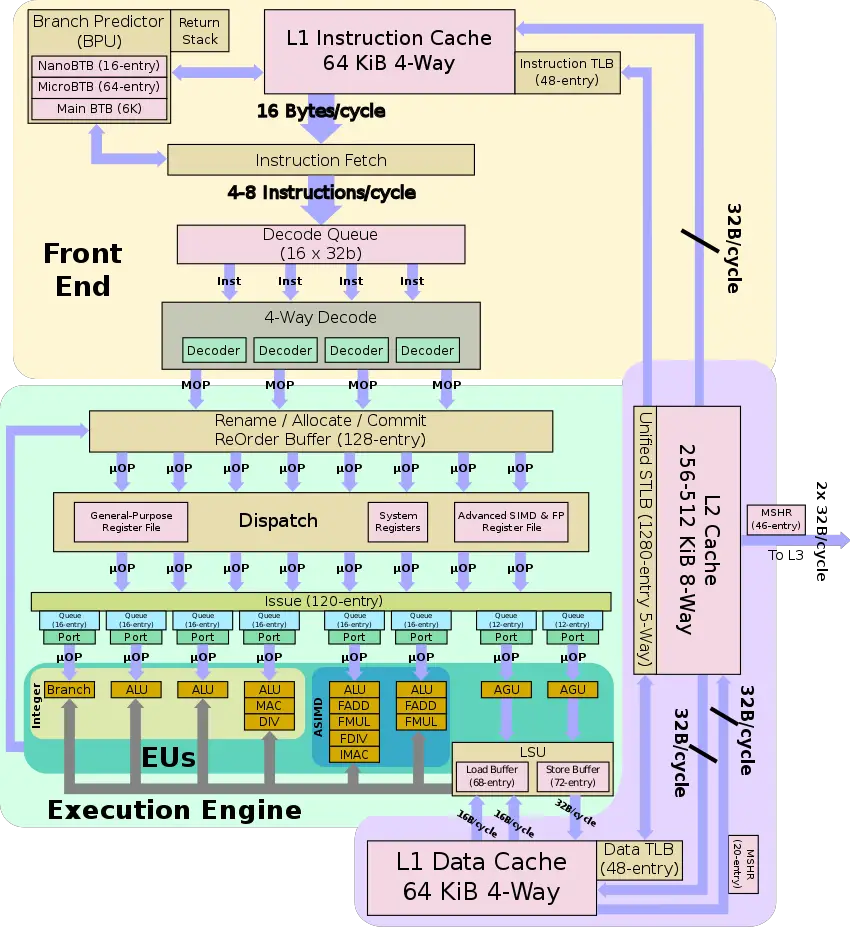
\includegraphics[width=0.8\linewidth]{Images/Cauce1.png}
    \caption{Cauce del procesador ARM cortex A76.}
    \label{fig:Cauce_ARM_cortex_a76}
\end{figure}

\begin{itemize}
    \item Como ya se comentaba en la Sección~\ref{subsec:repaso_ILP}, la etapa de ejecución y de memoria se consideraba una sola, al ser las instrucciones bien de acceso a memoria o bien instrucciones aritmético-lógicas.
    \item La etapa de emisión (aquella en la que ya se conocen los operandos y se prepara para mandar a ejecución) forma parte de la decodificación.
\end{itemize}

\subsection{Implementación de la emisión}
